\section{PROPOSED APPROACH}

This section describes the steps followed to build and evaluate the student at-risk prediction systems. The work was carried out in four stages: data collection and preprocessing, exploratory data analysis, model development, and evaluation. Each stage is described below, along with the reasoning behind the main decisions.

\subsection{Dataset and Scope}

The dataset used in this study comes from the Open University Learning Analytics Dataset (OULAD), a publicly available collection of anonymised records from a UK distance-learning university \parencite{kuzilek2017oulad}. OULAD contains information about students, their demographic backgrounds, their interactions with the Virtual Learning Environment (VLE), their assessment results, and their final outcomes across multiple course offerings.

The project was scoped specifically to module BBB, presentation 2013J, so that the students being analysed were exposed to the same course structure, assessment schedule, learning materials, and teaching period. In the OULAD dataset, different modules and presentations may differ in the number and timing of assessments, the weighting of coursework, the availability and structure of VLE activities, and the academic calendar. If multiple modules or presentations were combined, differences in student outcomes could be caused by these course-level differences rather than by the behavioural or academic risk factors used by the expert system. Limiting the scope therefore helps ensure that risk patterns such as low engagement, late registration, or weak continuous assessment performance are compared within a more consistent learning context.

Only the first fourteen weeks of each student's enrolment were used. This constraint served the early-prediction goal of the study. Using data from only the early part of a course means that any at-risk prediction could theoretically be acted upon while students still have time to receive support. Using data from the full course would allow the models to see information that is only available after the outcome has already been determined, which would defeat the practical purpose of prediction.

\subsection{Data Preprocessing}

Preprocessing was carried out using the R programming language \parencite{rcore2024} and the ouladFormat package, which provides tools for loading and combining the separate OULAD data tables into a single student-level dataset.

Repeat students were removed from the dataset. Students who had previously attempted the same module were excluded because their behaviour in a second attempt may be influenced by prior experience, making them different from first-time students in ways that are hard to model systematically. Withdrawn students were kept. Since the study aims to identify students who are likely to fail or withdraw, it was important that both groups appeared in the training data.

VLE engagement was measured through click counts. The OULAD dataset records how many times each student clicked on different types of learning materials. Rather than treating each activity type as a separate feature, all click counts were summed into a single variable called \texttt{total\_clicks}. This aggregation simplified the feature space and reduced the risk of creating too many sparse features from activity types that few students used.

Assessment performance was summarised using the \texttt{average\_CA\_score} variable, which represents the student's weighted average continuous assessment score for assessments due within the fourteen-week observation window. In the preprocessing script, missing or unavailable assessment marks were not removed; they were treated as zero in the weighted assessment calculation, which reflects the assumption that an assessment without a recorded grade contributes no achieved marks. Individual assessment columns identified only by numeric IDs were dropped because they are harder to interpret and harder to use meaningfully in rule-based systems.

Several columns were removed to prevent leakage or to avoid redundancy. The student ID was dropped because it is an identifier with no predictive meaning. The module and presentation codes were constant across the entire dataset and therefore carried no information. The number of previous attempts was constant after removing repeat students. The unregistration date was removed because it directly reveals whether a student withdrew, which would leak the target outcome into the input features.

After preprocessing, the final dataset contained one row per student and ten input features: \texttt{date\_registration}, \texttt{gender}, \texttt{region}, \texttt{highest\_education}, \texttt{imd\_band}, \texttt{age\_band}, \texttt{studied\_credits}, \texttt{disability}, \texttt{average\_CA\_score}, and \texttt{total\_clicks}. The outcome variable \texttt{final\_result} was retained as the raw label and later converted into the binary prediction target.

\subsection{Exploratory Data Analysis}

Before building any models, an exploratory data analysis (EDA) was performed using Python and the pandas and matplotlib libraries \parencite{mckinney2010pandas,hunter2007matplotlib}. The purpose of the EDA was to answer specific questions that would guide the preprocessing and modelling decisions in the next stage.

The first question was whether the target classes were balanced or not. As shown in Figure~\ref{fig:target_distribution}, the target variable does not exhibit a significant class imbalance. The class distribution is approximately 66:33, which is considered acceptable, as both classes contain a sufficient number of samples.

\begin{figure}[htbp]
    \centering
    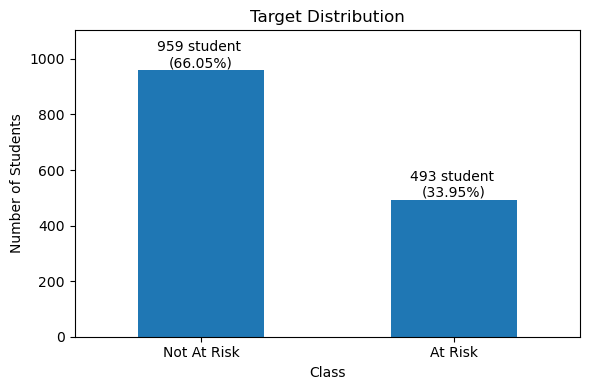
\includegraphics[width=0.8\textwidth]{figures/target_distribution.png}
    \caption{Target distribution of OULAD dataset}
    \label{fig:target_distribution}
\end{figure}

The second question was whether the input features showed any clear relationship with the at-risk outcome. For each feature, the distribution of at-risk and not-at-risk students was plotted. Numeric features such as \texttt{average\_CA\_score}, \texttt{total\_clicks}, and \texttt{date\_registration} were grouped into quantile bins before plotting so that the comparison was not distorted by extreme values. Categorical features such as \texttt{imd\_band} and \texttt{highest\_education} were plotted directly, with each category shown as a separate group.

As shown in Figure~\ref{fig:target_distribution_by_average_CA_score}, as the accumulated assessment scores increase, the number of At Risk (Class 1) students decreases, while the number of Not At Risk (Class 0) students increases. This is entirely expected, as a student who performs well in previous assessments is likely to perform well in the final exam as well, and vice versa.

\begin{figure}[htbp]
    \centering
    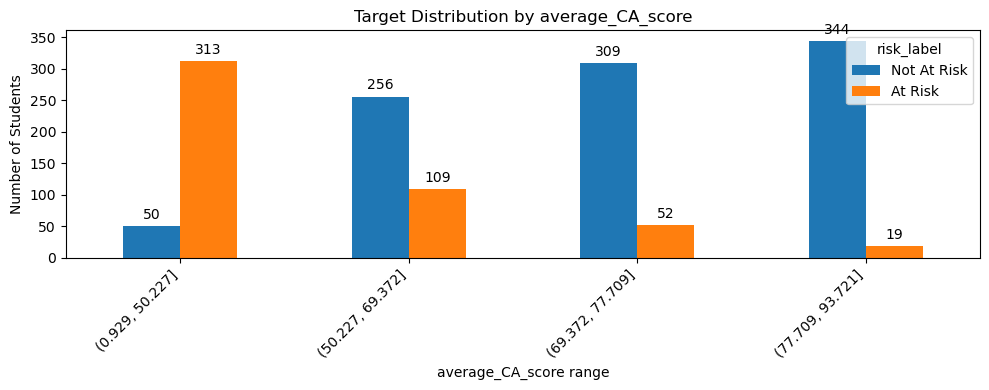
\includegraphics[width=0.8\textwidth]{figures/target_distribution_by_average_CA_score.png}
    \caption{Target distribution by average\_CA\_score}
    \label{fig:target_distribution_by_average_CA_score}
\end{figure}

Similarly, Figure~\ref{fig:target_distribution_by_total_clicks} also has a direct relation with the target. The number of At Risk students decreases, while the number of Not At Risk students increases, as student engagement with the VLE increases. Students who are more engaged with the learning platform and course materials are more likely to study consistently and, consequently, achieve higher final results.

\begin{figure}[htbp]
    \centering
    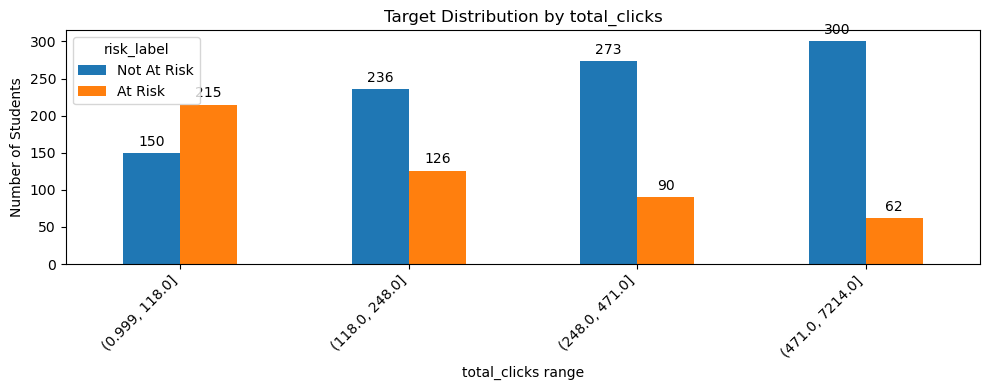
\includegraphics[width=0.8\textwidth]{figures/target_distribution_by_total_clicks.png}
    \caption{Target distribution by total\_clicks}
    \label{fig:target_distribution_by_total_clicks}
\end{figure}

Figure~\ref{fig:target_distribution_by_imd_band} also shows that the higher values for \texttt{imd\_band}, which represents the Index of Multiple Deprivation band and serves as an indicator of socioeconomic background, are associated with a low number of At Risk students. This relation is expected, as students from more advantaged socioeconomic backgrounds often have greater access to educational resources, such as private tutoring and supportive learning environments, which can contribute to improved academic performance and a lower risk of failure.

\begin{figure}[htbp]
    \centering
    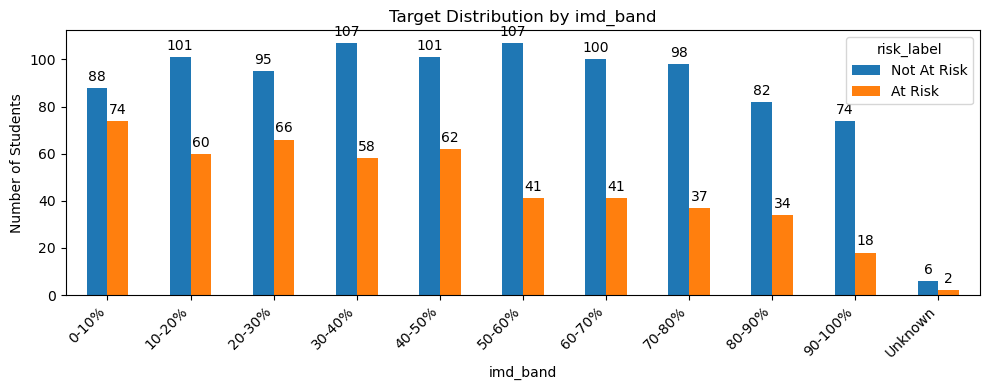
\includegraphics[width=0.8\textwidth]{figures/target_distribution_by_imd_band.png}
    \caption{Target distribution by imd\_band}
    \label{fig:target_distribution_by_imd_band}
\end{figure}

Figure~\ref{fig:target_distribution_by_highest_education} shows a clear relationship between a student's prior educational attainment and their likelihood of being classified as At Risk. Students with qualifications lower than A-Level exhibit the highest proportion of At Risk cases (263 out of 341 students, approximately 77.1\%). This proportion decreases for students with A-Level or equivalent qualifications (182 out of 479 students, approximately 38.0\%) and is lowest among students holding a Higher Education (HE) qualification (42 out of 130 students, approximately 32.3\%). This trend suggests that students with stronger educational backgrounds are less likely to be at risk, likely because prior academic experience equips them with the knowledge, study skills, and learning strategies necessary to succeed in their courses.

\begin{figure}[htbp]
    \centering
    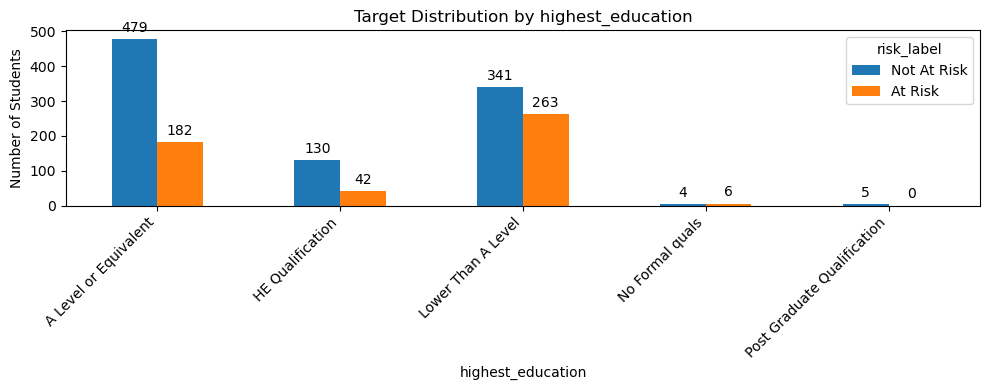
\includegraphics[width=0.8\textwidth]{figures/target_distribution_by_highest_education.png}
    \caption{Target distribution by highest\_education}
    \label{fig:target_distribution_by_highest_education}
\end{figure}


The third question was whether any features had missing values that would need to be handled before modelling. \texttt{imd\_band} had a small number of missing values. These were addressed in later preprocessing by treating them as a separate category rather than imputing a numeric substitute, since the variable is categorical.


\subsection{Target Definition and Feature Selection}

Before training any model, the outcome variable \texttt{final\_result} was converted into a binary target. Students whose final result was either Fail or Withdrawn were labelled as At Risk (class 1). Students whose result was Pass or Distinction were labelled as Not At Risk (class 0). This mapping was chosen because both failure and withdrawal represent outcomes where the student did not successfully complete the module, and both are outcomes that early intervention could potentially help to prevent.

Feature selection was carried out before model training by retaining only variables that could be interpreted as early registration, demographic/background, academic-performance, or engagement indicators. The selected numeric features were \texttt{date\_registration}, \texttt{average\_CA\_score}, and \texttt{total\_clicks}. The selected categorical or background features were \texttt{gender}, \texttt{region}, \texttt{highest\_education}, \texttt{imd\_band}, \texttt{age\_band}, \texttt{studied\_credits}, and \texttt{disability}. These variables matched the feature groups used in the modelling notebook: registration, academic performance, engagement, and demographics/background.

Features were excluded when they were identifiers, constants within the selected scope, difficult to interpret in rule form, or likely to leak the target. The student ID was removed because it has no predictive meaning. The module and presentation codes were removed because all rows came from BBB/2013J. Individual assessment ID columns were removed after deriving \texttt{average\_CA\_score}. \texttt{date\_unregistration} was removed because it directly reveals withdrawal and would therefore leak the at-risk outcome into the model inputs.

\subsection{Train/Test Split}

The dataset was divided into training and test sets using an 80:20 split. The split was stratified based on the target variable to ensure that the class distribution was preserved across both sets and to avoid potential class imbalance.

The same training set and test set were used for all three systems: the expert system, the logistic regression model, and the support vector machine. Using identical splits ensured that the performance differences observed between the systems reflected genuine differences in how the systems reason, rather than differences caused by one system seeing easier or harder students.

A fixed random seed (42) was set throughout the notebook so that results were fully reproducible.

\subsection{Expert System Development}

The expert system was built in three steps: preprocessing for rule generation, decision tree training for rule extraction, and deployment of the rules inside an Experta inference engine.

\subsubsection{Preprocessing for the Expert System}

Categorical features were preprocessed by replacing missing values with an explicit Unknown category and then applying one-hot encoding. This was necessary because the decision tree used for expert-system rule generation requires numeric input, while features such as \texttt{gender}, \texttt{region}, \texttt{highest\_education}, \texttt{imd\_band}, \texttt{age\_band}, and \texttt{disability} are categorical. Using Unknown allowed missing values to be retained as a visible category rather than removing records or making assumptions about the missing data.

One-hot encoding converted each category into a separate binary column, with values of 0 or 1. This avoided giving categories an artificial numerical order. For example, assigning numbers to regions or education levels could incorrectly suggest that one category is greater than another. One-hot encoding preserved the meaning of each category and also made the extracted rules easier to interpret, because each binary feature could be translated directly into a clear condition, such as whether a student belonged to a particular IMD band or education group.

\subsubsection{Decision Tree Rule Generation}

A decision tree classifier was trained on the preprocessed training data \parencite{breiman1984classification}. The purpose of this decision tree was not to serve as the final prediction model. Its sole purpose was to discover a set of meaningful IF-THEN rules that could be transferred into the expert system's knowledge base.

The tree was configured with specific settings chosen to produce clean, readable rules rather than maximum predictive accuracy. The maximum depth was set to four, which limits each rule to at most four conditions. Deeper trees can capture more complex patterns but also produce rules with many conditions that are harder to interpret and more likely to be specific to the training data. The minimum number of samples required to split a node was set to ten, and the minimum number of samples in a leaf was set to five, which prevents the tree from generating rules that apply to only one or two students. The splitting criterion was information entropy, which measures how much a split reduces the uncertainty about the outcome. Class weights were set to balanced to give proportionally more importance to at-risk students during training, since they were the minority class and missing them was the more harmful type of error.

The tree produced fourteen rules, one for each leaf node. Each leaf represented one complete path from the root of the tree to a terminal node, and the prediction at each leaf was the majority class among the training samples that reached that node, as shown in Figure~\ref{fig:decision_tree_from_rules}.

\begin{figure}[htbp]
    \centering
    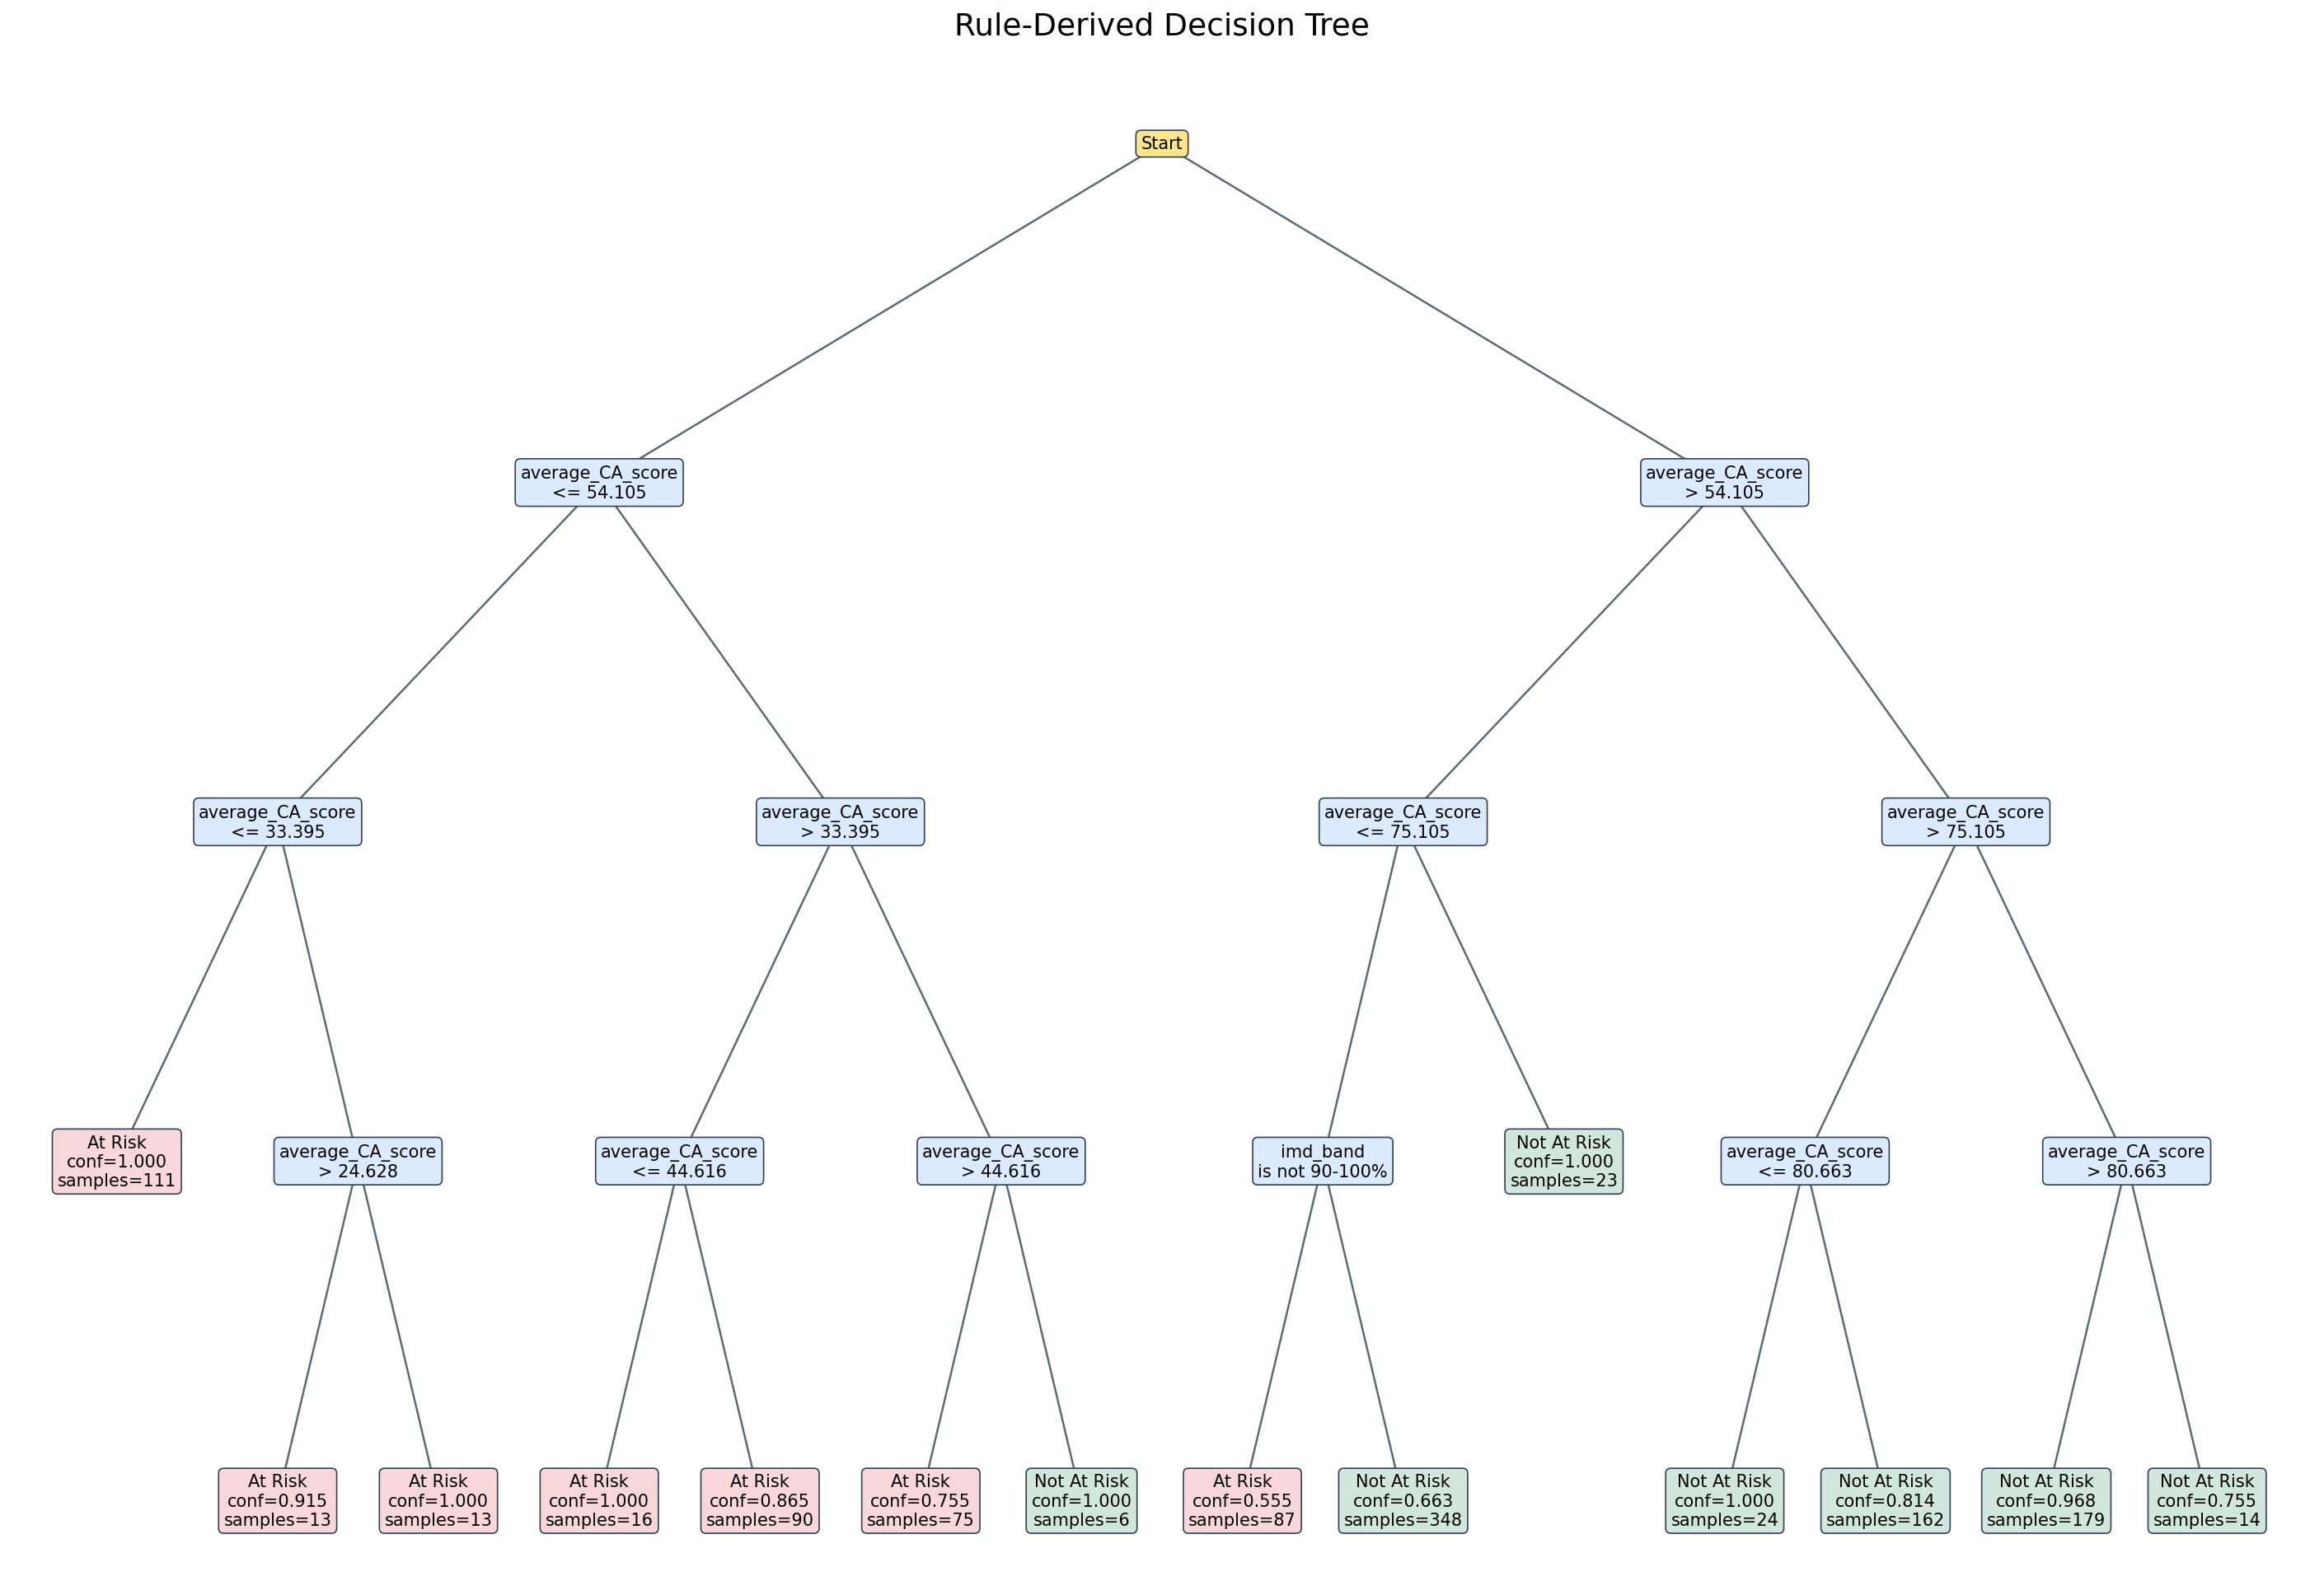
\includegraphics[width=0.8\textwidth]{figures/decision_tree_from_rules.png}
    \caption{Derived Rules as a Decision Tree}
    \label{fig:decision_tree_from_rules}
\end{figure}

\subsubsection{Knowledge Base Construction}

Each leaf path was extracted from the trained decision tree and converted into a structured IF-THEN rule. Each rule stored the list of conditions, the predicted class (At Risk or Not At Risk), the confidence (the proportion of training samples at that leaf that belonged to the predicted class), and the number of training samples that reached the leaf. For conditions involving one-hot encoded features, the binary threshold was translated back into a readable form. For example, a condition that checked whether the \texttt{imd\_band\_90-100\%} column was greater than 0.5 was written as ``imd\_band is 90-100\%'' rather than keeping the numeric encoding visible.

The generated rule base showed that \texttt{average\_CA\_score} was the dominant condition used for risk classification, appearing across most of the extracted rules. This indicates that early continuous assessment performance was the main factor used by the expert system to separate At Risk and Not At Risk students. Other features, such as \texttt{total\_clicks}, \texttt{date\_registration}, and \texttt{imd\_band}, appeared less frequently and were mainly used to refine classifications for students whose assessment scores fell within intermediate ranges.

\subsubsection{Experta Inference Engine}

The knowledge base was deployed inside a rule-based inference engine built with the Experta library \parencite{experta2015}. Experta is a Python framework for building expert systems using a fact-and-rule architecture. Each student in the test set was represented as a Student fact containing the student's preprocessed feature values. When a student fact was added to the engine, the engine iterated through all fourteen knowledge base rules and identified the one rule whose conditions all matched the student's values. Since the rules were derived from a decision tree -- where every input follows exactly one path from root to leaf -- exactly one rule matched each student. The matched rule's prediction was recorded as the expert system's output for that student.

\subsection{Machine Learning Baselines}

Two machine learning models were used as baselines for comparison with the expert system: Logistic Regression (LR) and a Support Vector Machine (SVM) with a radial basis function (RBF) kernel \parencite{cortes1995support}.

Both models used the same selected input features and the same train/test split as the expert system. However, their preprocessing pipeline was different in one important respect: numeric features were standardised using z-score scaling before being passed to the models. Scaling was necessary because both LR and SVM are sensitive to the magnitude of input values. A feature measured in hundreds (such as \texttt{total\_clicks}) would dominate a feature measured in single digits (such as \texttt{date\_registration}) if both were passed in their original form. Standardisation puts all numeric features on the same scale, ensuring that the models treat each feature on equal terms.

The logistic regression model was configured with a maximum of 5,000 iterations to ensure convergence on this dataset and with balanced class weights to compensate for the imbalanced target distribution. The SVM used an RBF kernel, which maps the data into a higher-dimensional space to find a decision boundary that is not necessarily linear. It was also configured with balanced class weights.

Logistic Regression and SVM were trained using preprocessing pipelines rather than manually preprocessed feature matrices. The selected training data was passed into each pipeline with categorical features still in their original label form. Within the pipeline, missing values were imputed, categorical variables were one-hot encoded, and numeric variables were scaled before the classifier was fitted. This design meant that training a model required only one call, and the preprocessing steps were always applied in the correct order \parencite{pedregosa2011scikit}.

\subsection{Evaluation}

All three systems -- the expert system, Logistic Regression, and the Support Vector Machine -- were evaluated on the same held-out test set. Accuracy was reported as an overall measure of classification performance, while precision, recall, and F1-score were calculated for the positive class (At Risk).

Accuracy: the proportion of all students whose risk status was predicted correctly, including both At Risk and Not At Risk cases.

Precision: of all students predicted to be at risk, the proportion who actually were at risk. High precision means fewer false alarms.

Recall: of all students who were actually at risk, the proportion who were correctly identified. High recall means fewer at-risk students are missed.

F1-score: the harmonic mean of precision and recall, which balances both concerns into a single number.

A confusion matrix was also produced for each system, showing how many students fell into each combination of actual and predicted class.

In educational risk prediction, recall is often considered the most practically important metric, because missing a student who is genuinely at risk has more serious consequences than generating a false alert for a student who is performing adequately. The evaluation therefore paid particular attention to recall when comparing the three systems.
